
\appendix


\chapter{Templates}

This section describes the templates used for creating the use case descriptions.

% <<< %%%%%%%%%%%%%%%%%%%%%%%%%%%%%%%%%%%%%%%%%%%%%%%%%%%%%%%%%%%%%%%%%%%%%%%%%%%%%%%%
\subsection{System: Template}
\label{System: Template}



\begin{figure} [htb]
	\centering
	\framebox{Architecture diagram}
	\caption{}
	\label{fig:uc generic data}
\end{figure}


\paragraph{System Description:}
A short description of the system/subsystem.
%Maybe half a page for a complex system.

\paragraph{Risks:}
\begin{itemize}
	\item A list of risk factors for the system
	\item ordered by priority
\end{itemize}


\paragraph{Subsystems:} A brief list of subsystems with a short description.

\begin{itemize}
	\item Subsystem 1: Really brief description.
	\item Subsystem 2: Really brief description.
	\item Subsystem 3: Really brief description.
\end{itemize}
% >>> %%%%%%%%%%%%%%%%%%%%%%%%%%%%%%%%%%%%%%%%%%%%%%%%%%%%%%%%%%%%%%%%%%%%%%%%%%%%%%%%


%%%%%%%%%%%%%%%%%%%%%%%%%%%%%%%%%%%%%%%%%%%%%%%%%%
\section{Use Cases}

% <<< %%%%%%%%%%%%%%%%%%%%%%%%%%%%%%%%%%%%%%%%%%%%%%%%%%%%%%%%%%%%%%%%%%%%%%%%%%%%%%%%
\subsection{UC: Template}

This section is the general template for use cases.
Sections that do not apply may be dropped.

\paragraph{Actors:}
\begin{itemize}
	\item Which systems are involved?
	\item What kind of users are doing this? Scientists, Operators, Vendors?
\end{itemize}

\paragraph{Use-Case Description:}
A brief description of the scenario.
Why is it relevant?

Which subsystems maybe affected?
Which objectives matter most?

\paragraph{Priority:}
High, Middle, Low -- Short explanation.. e.g., x\% of workload seen


\paragraph{Data/Domain Description:}
A description and if possible an illustration of the data structure, for example:
How is the domain defined (1d, 2d, 3d, ...)?
What kind of grid?
Is it a time series?
Array of structures vs. structure of Arrays?
Mostly input/output?
Expected data volumes?

\paragraph{Domain Decomposition:}
\begin{itemize}
	\item Node level domain decomposition
	\item Storage level domain decomposition/data segmentation
\end{itemize}

\begin{figure} [htb]
	\centering
	\framebox{Illustration of the data domain inside the parallel application.}
	%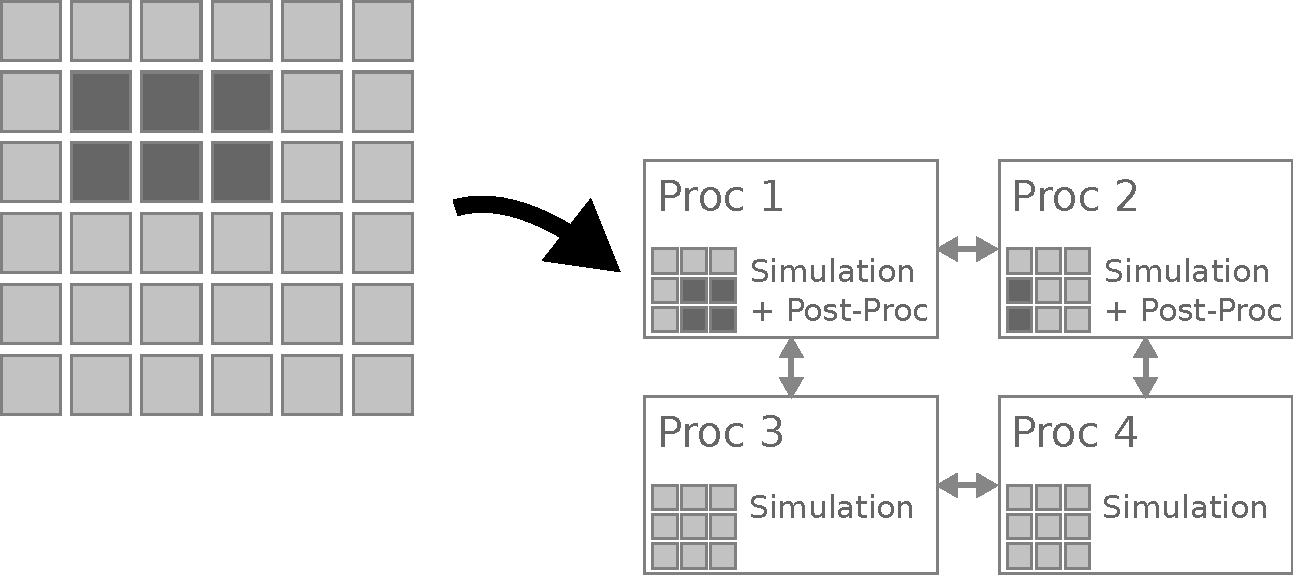
\includegraphics[width=0.5\linewidth]{use-cases/uml/USE+CASE+NAME/domain}
	\caption{Domain Illustration}
	\label{fig:domain template}
\end{figure}


\paragraph{Pre-Conditions:}
\begin{itemize}
	\item What needs to be true before a use case starts?
\end{itemize}

\paragraph{Post-Conditions:}
\begin{itemize}
	\item What should be true after the use case finishes?
\end{itemize}



\paragraph{Used Use-Cases:}
\begin{itemize}
	\item Are any other use-cases used? List here. / Split use case in case they get to complex
\end{itemize}


\paragraph{Flow of Events:}
\begin{enumerate}
	\item Component A: Action
	\item Component B: Another action.
\end{enumerate}


\begin{figure} [htb]
	\centering
	\framebox{Activity diagram illustrating the actors and their high-level operations}
	%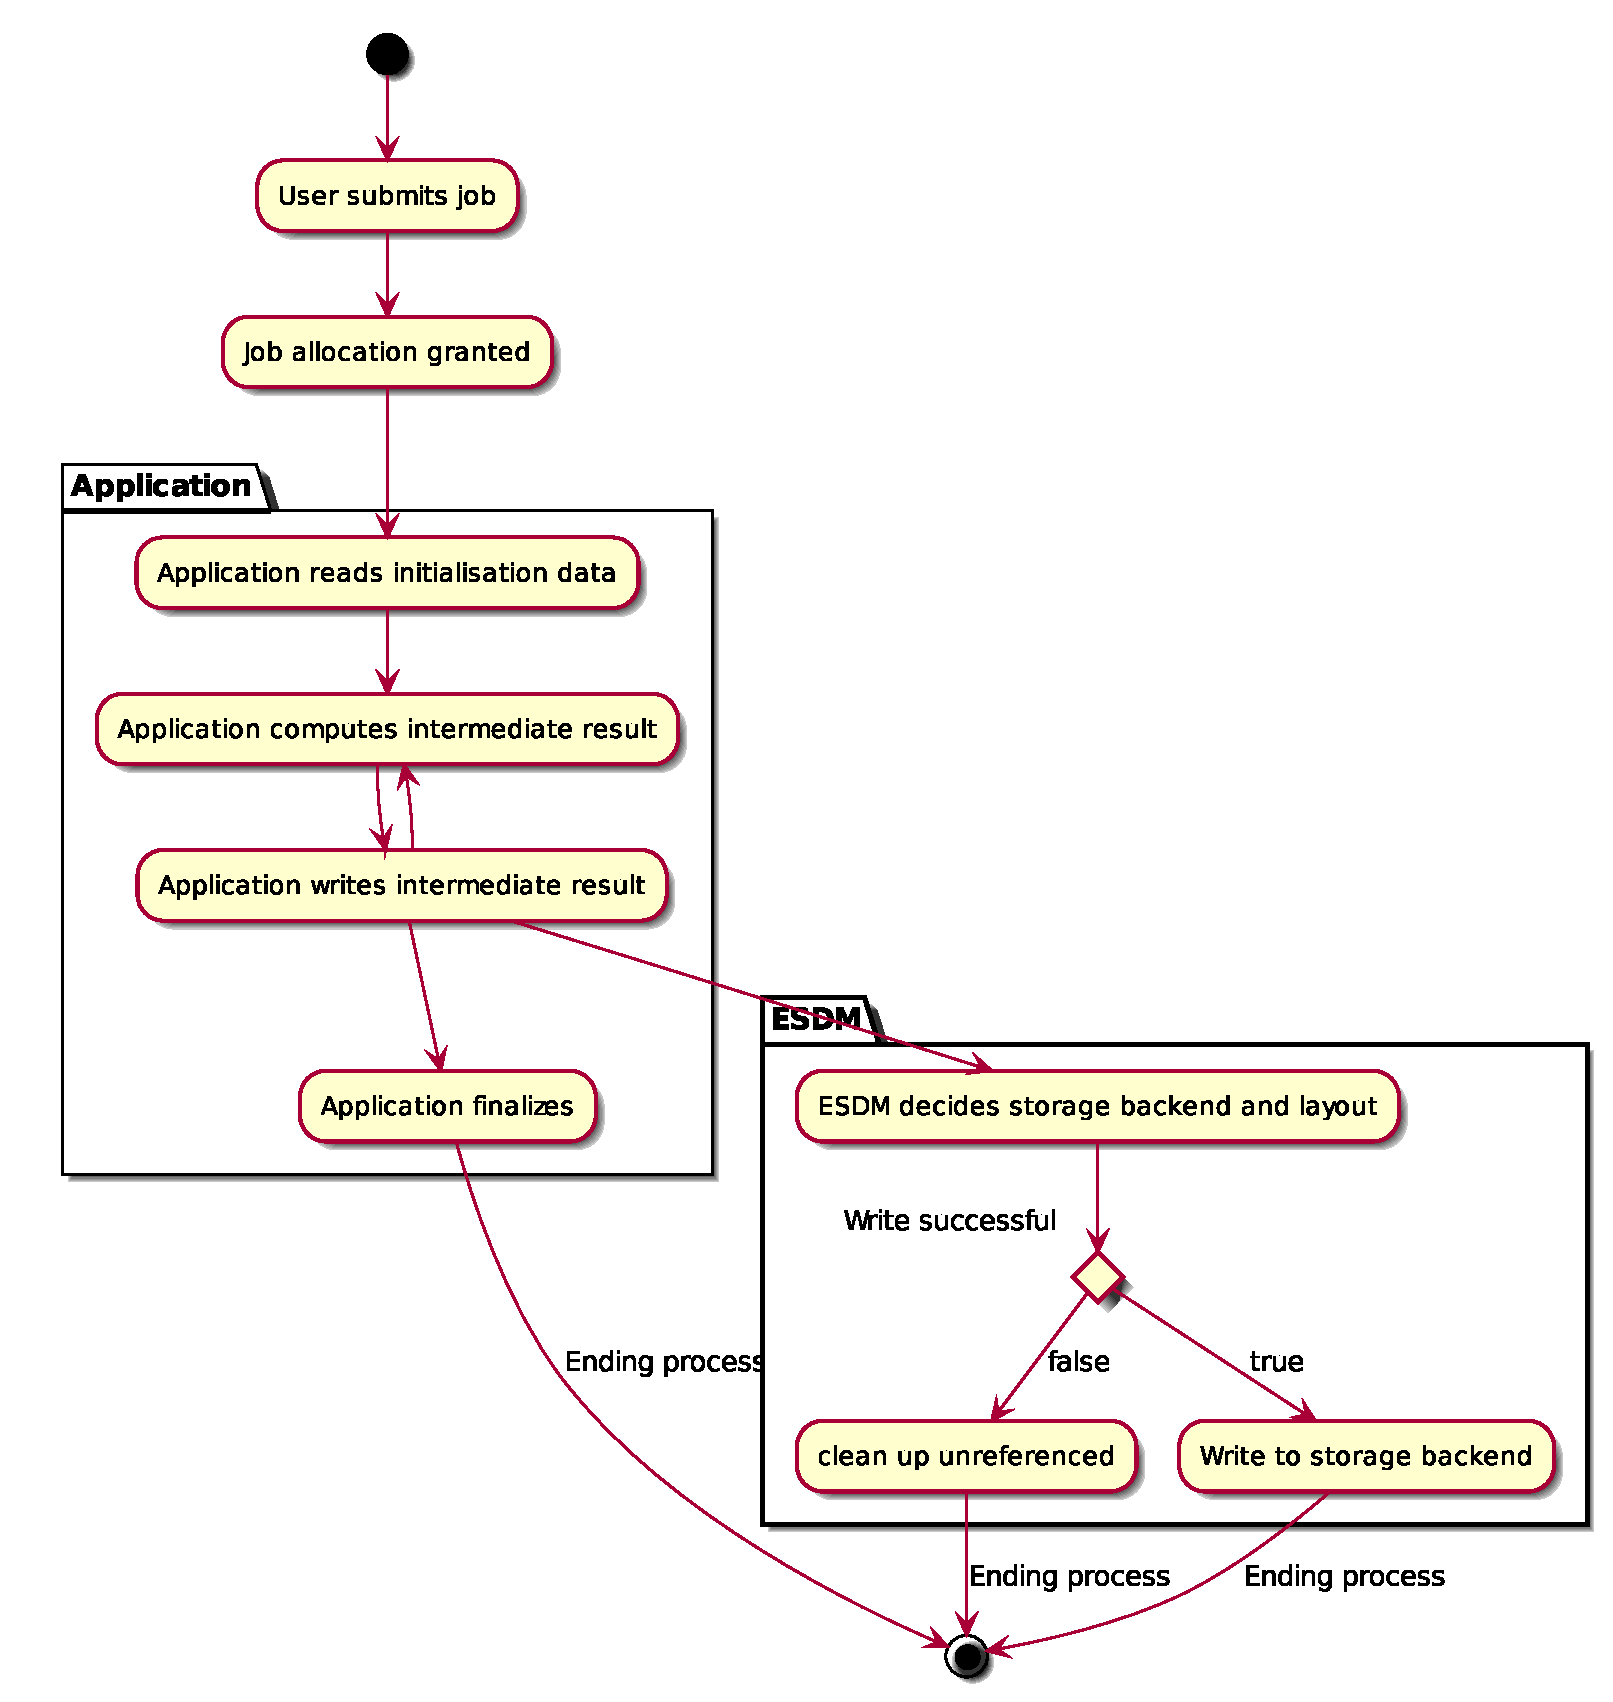
\includegraphics[width=0.5\linewidth]{use-cases/uml/USE+CASE+NAME/activity.eps}
	\caption{Activity Diagram}
	\label{fig:activity template}
\end{figure}

\paragraph{Exceptions:}
\begin{itemize}
	\item Scenario 1: Brief description.
	\item Scenario 2: Brief description.
\end{itemize}


\begin{figure} [htb]
	\centering
	\framebox{Sequence diagram showing the interactions of the individual components}
	%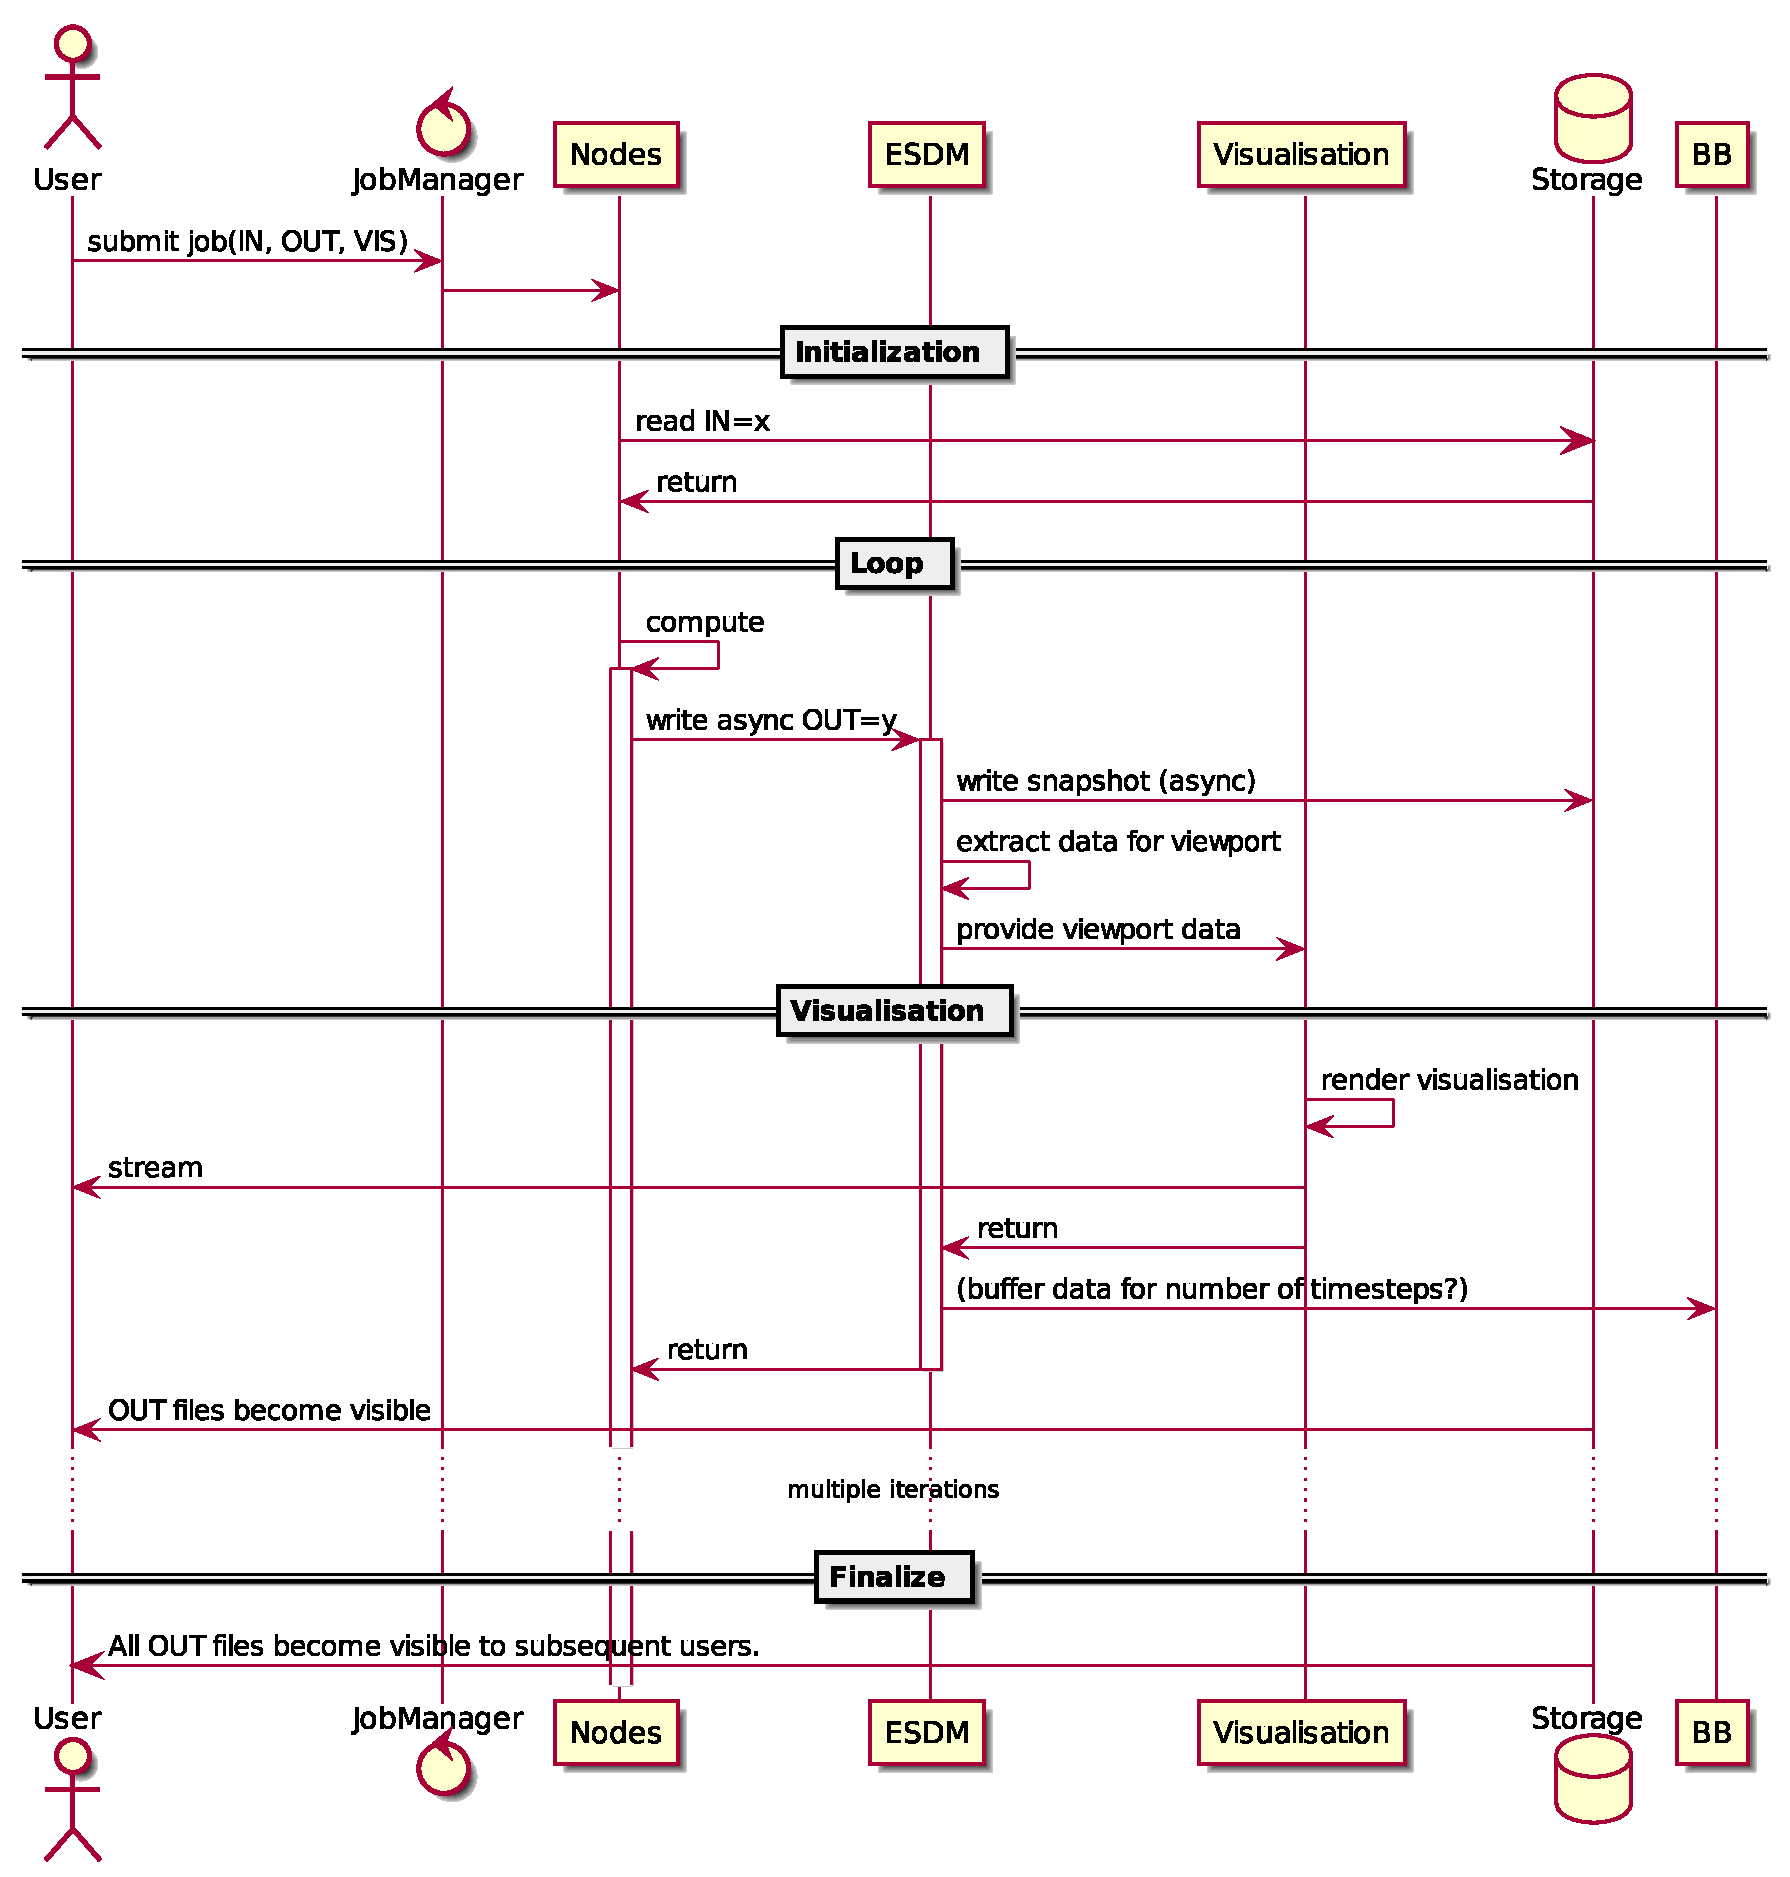
\includegraphics[width=0.5\linewidth]{use-cases/uml/USE+CASE+NAME/sequence.eps}
	\caption{Sequence Diagram}
	\label{fig:sequence template}
\end{figure}


%\paragraph{Subordinate Use-Cases:}
%\begin{itemize}
%	\item For special cases that are not adequate as a scenario. If any.
%\end{itemize}


\begin{figure} [h]
	\centering
	\framebox{Participating objects}
	%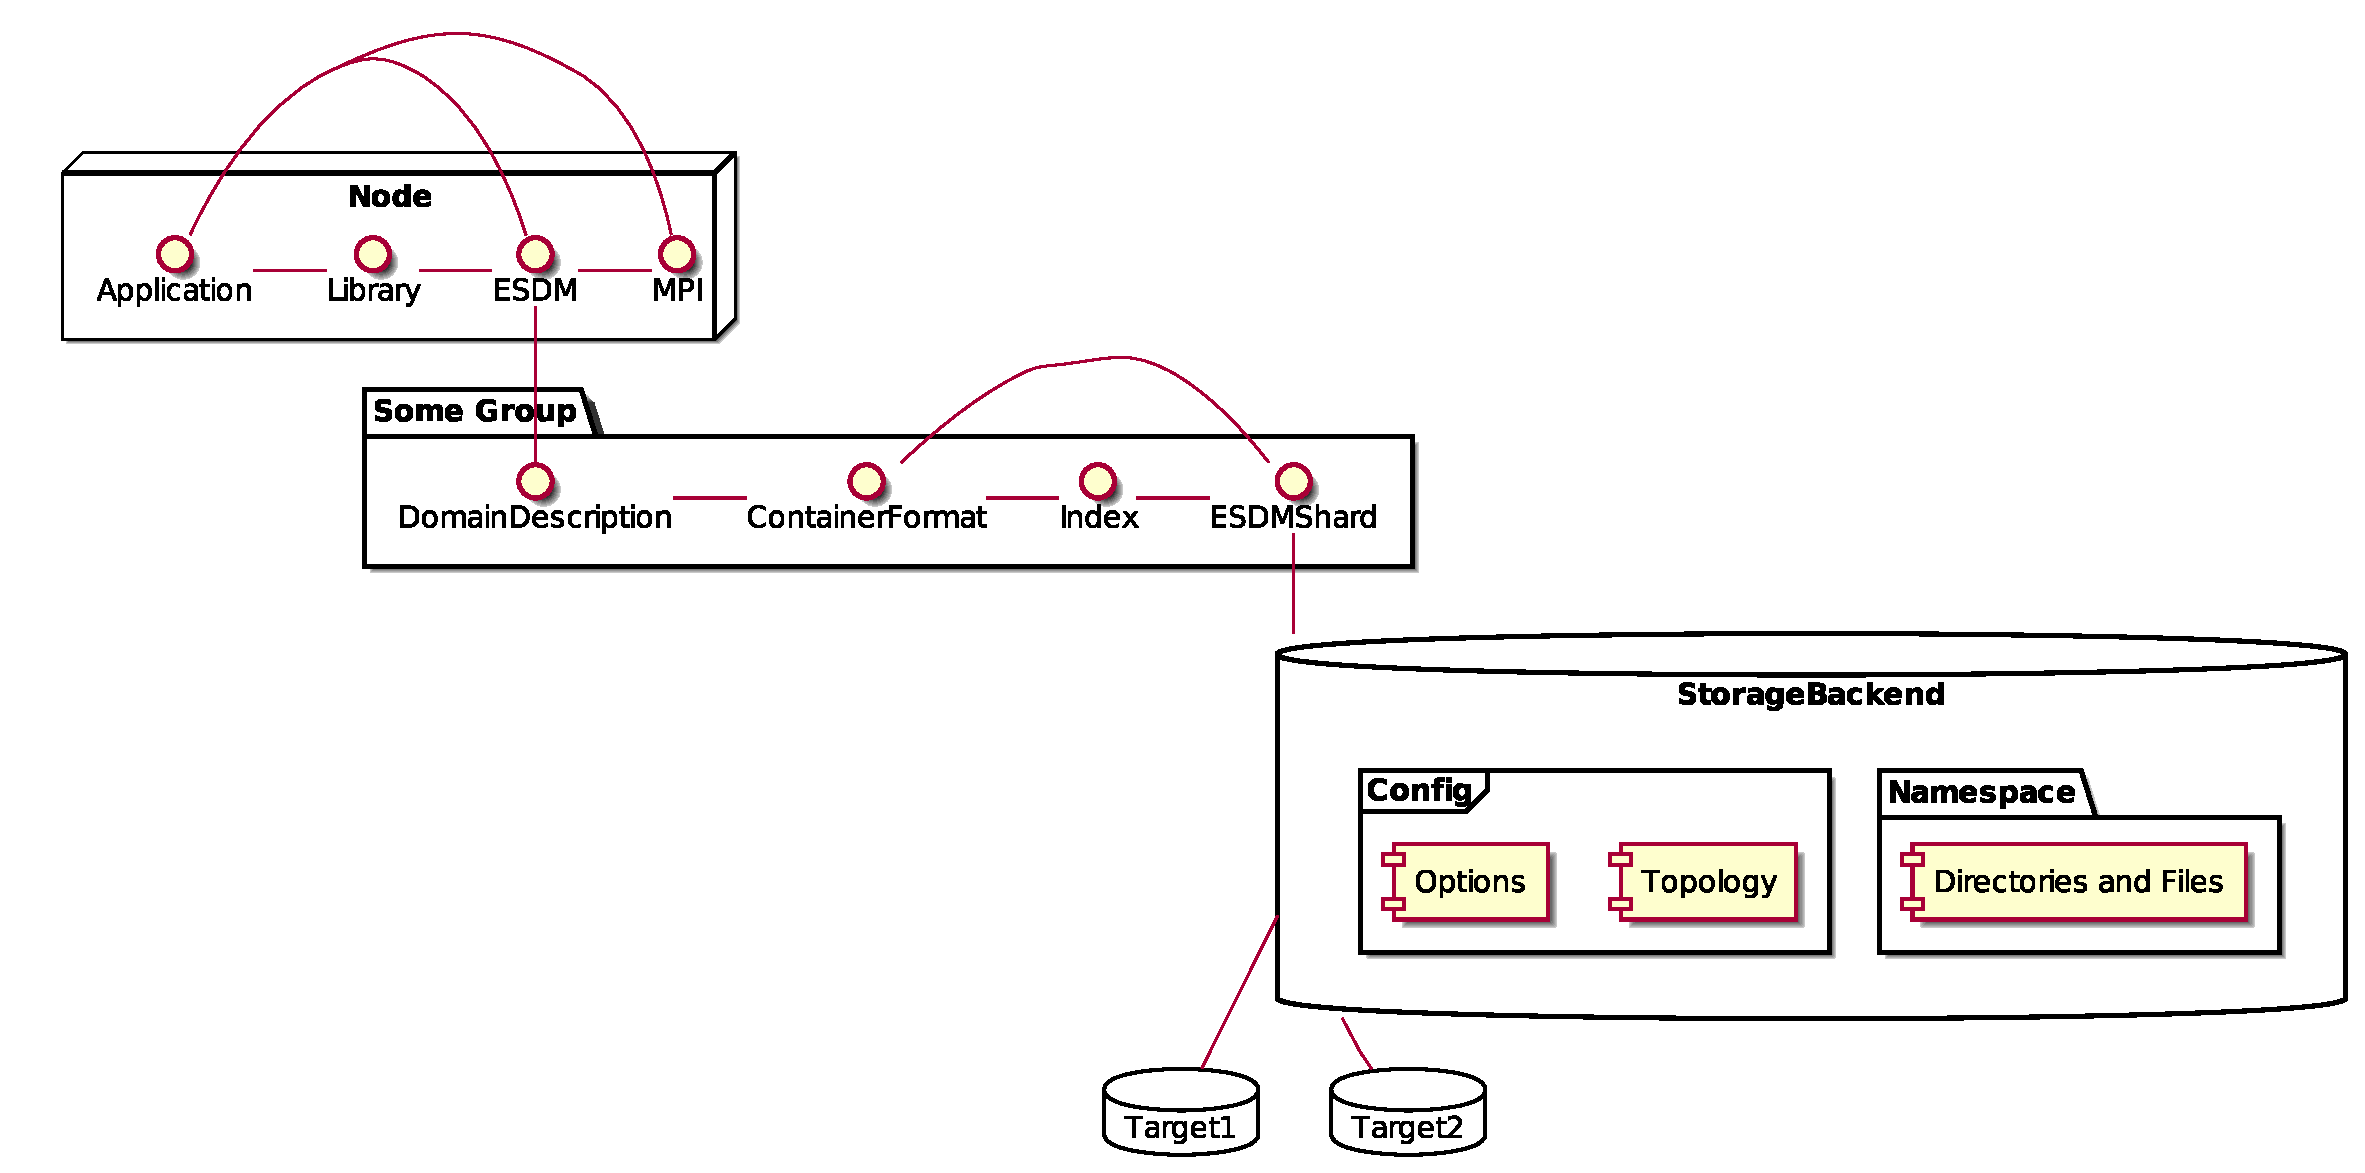
\includegraphics[width=0.5\linewidth]{use-cases/uml/USE+CASE+NAME/participants.eps}
	\caption{Participating Objects}
	\label{fig:objects template}
\end{figure}



\paragraph{Assumptions:}
Any assumptions that have been made, besides pre-conditions and post conditions that are notable.


\paragraph{Notes/Issues:}
Room for notes. Are there known issues?



% <<< %%%%%%%%%%%%%%%%%%%%%%%%%%%%%%%%%%%%%%%%%%%%%%%%%%%%%%%%%%%%%%%%%%%%%%%%%%%%%%%%
